\documentclass[10pt,xcolor=pdflatex]{beamer}
\usepackage{newcent}
\usepackage[utf8]{inputenc}
\usepackage[slovak]{babel}
\usepackage{hyperref}
\usepackage{fancyvrb}
\usepackage{multirow}
\usetheme{FIT}

%%%%%%%%%%%%%%%%%%%%%%%%%%%%%%%%%%%%%%%%%%%%%%%%%%%%%%%%%%%%%%%%%%
\title[Metody extrakce dat z webových stránek]{Metody extrakce dat z~webových~stránek}

\author[]{Lukáš Perina}

\institute[]{Brno University of Technology, Faculty of Information Technology\\
Bo\v{z}et\v{e}chova 1/2. 612 66 Brno - Kr\'alovo Pole\\
xperin11@fit.vutbr.cz}

\date{Jún 16, 2021}
%\date{\today}
%\date{} % bez data

%%%%%%%%%%%%%%%%%%%%%%%%%%%%%%%%%%%%%%%%%%%%%%%%%%%%%%%%%%%%%%%%%%

\begin{document}

\frame[plain]{\titlepage}

\begin{frame}\frametitle{Motivácia}
    \begin{itemize}
        \item Extrakcia dát z webu stále nieje dokonalá
        \bigskip
        \item Možnosť extrakcie na základe uvedenia \emph{obsahu} webového dokumentu
        \bigskip
        \item Automatizácia
    \end{itemize}
\end{frame}

\begin{frame}\frametitle{Technológie súčasnosti}
    \begin{itemize}
        \item Hotové riešenia
        \bigskip
            \begin{itemize}
                \item Scrapping-bot
                \smallskip
                \item Octoparse
                \smallskip
                \item Import.io
            \end{itemize}
        \bigskip
        \item Platformy a knižnice
        \bigskip
            \begin{itemize}
                \item Apify SDK
                \smallskip
                \item Cheerio
                \smallskip
                \item Scrapy
                \smallskip
                \item \emph{Puppeteer}
            \end{itemize}
    \end{itemize}
\end{frame}

\begin{frame}\frametitle{Návrh architektúry}
    \begin{figure}[hbt]
    	\centering
    	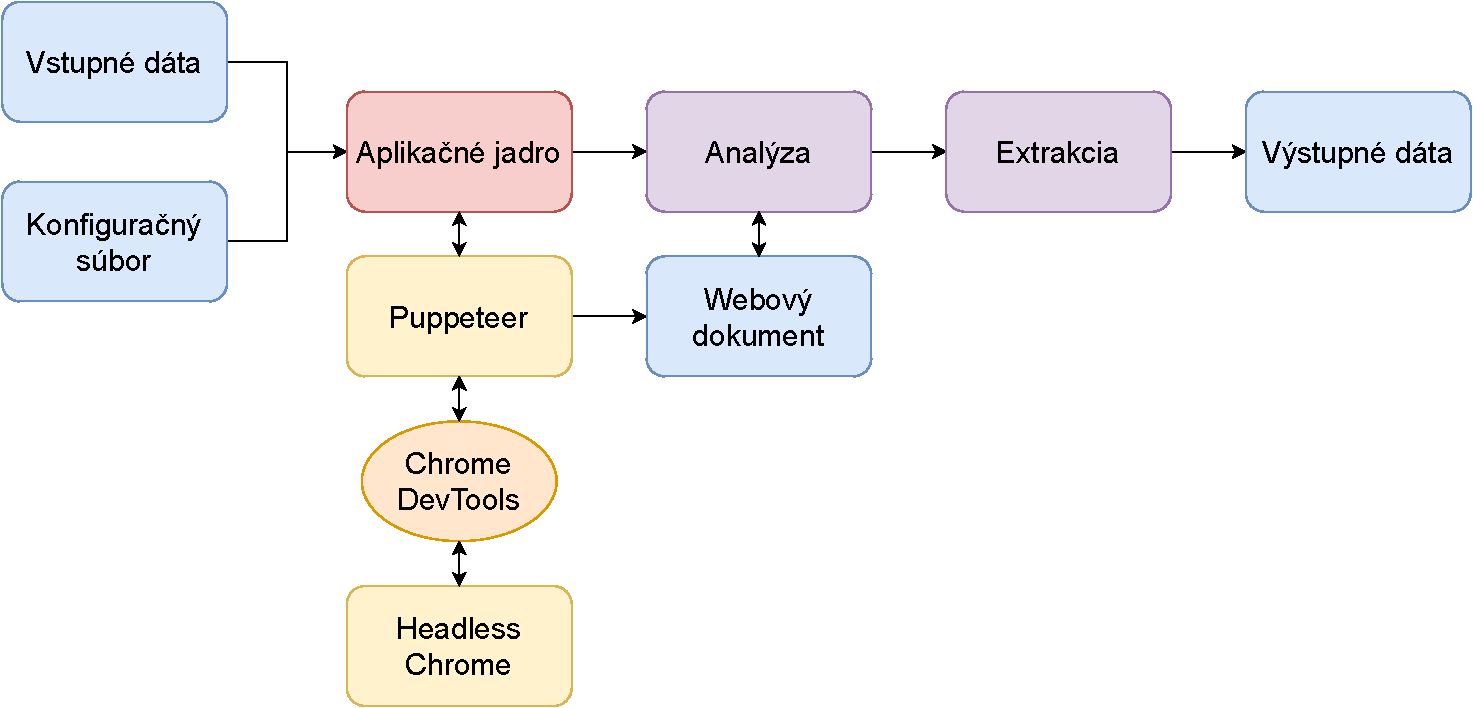
\includegraphics[width=0.9\textwidth]{img/architecture.pdf}
    	\caption{Diagram navrhnutej architektúry}
    \end{figure}
\end{frame}

\begin{frame}\frametitle{Implementácia}
    \begin{itemize}
        \item Konfiguračný súbor
        \bigskip
        \item Vstupné dáta
        \bigskip
        \item Analýza a extrakcia
        \bigskip
            \begin{itemize}
                \item Analýza štylizačných atribútov \emph{class}
                \bigskip
                \item Zoradenie na základe početnosti
                \bigskip
                \item Detekcia primárneho prvku
                \bigskip
                \item Zostavenie \emph{stromovej štruktúry} a následná extrakcia dát
            \end{itemize}
    \end{itemize}
\end{frame}

\begin{frame}\frametitle{Vyhodnotenie výsledkov}
    \bgroup
    \def\arraystretch{1.5}
    \begin{table}[hbt]
        \caption{Výsledné hodnoty testovaných dátových sád}
        \centering
        \begin{tabular}{|l|l|l|l|l|l|l|}
        \hline
        \textbf{Dátová sada}          & \textbf{Presnosť} & \textbf{Úplnosť}  & \textbf{Čas} \\ \hline
        Futbalové výsledky   & 97,9 \%   & 86,5 \%  & 13627 ms \\ \hline
        Eshop TSBohemia      & 100,0 \%  & 100,0 \% & 10876 ms \\ \hline
        Eshopy               & 71,42 \%  & 68,41 \% & 11228 ms \\ \hline
        Správy a novinky     & 72,73 \%  & 66,23 \% & 12885 ms \\ \hline \hline \hline
        \textbf{Priemerné výsledky}  & 85,51 \%  & 80,28 \% & 12154 ms \\ \hline
        \end{tabular}
    \end{table}
    \egroup
    \emph{Pozn.:} Dátová sada obsahuje 10 webových dokumentov.
\end{frame}

\begin{frame}\frametitle{Otázky oponenta}
    \begin{enumerate}
        \item U knihovny Puppeteer jste zmiňoval především výhody, můžete se zamyslet i nad nevýhodami použití této knihovny?
        \bigskip
        \item Chápu, že v současné době není k dispozici žádná srovnávací testovací sada pro alternativní nástroje, ale dle zmínky v textu byl vytvořen jiným studentem alternativní nástroj s jiným přístupem k extrakci, ale využívající stejné testovací sady. Můžete provést alespoň srovnání s kolegou z hlediska přesnosti a časové náročnosti pro jednotlivé sady?
    \end{enumerate}
\end{frame}

\begin{frame}\frametitle{Porovnanie aplikácií}
    \begin{figure}[hbt]
    	\centering
    	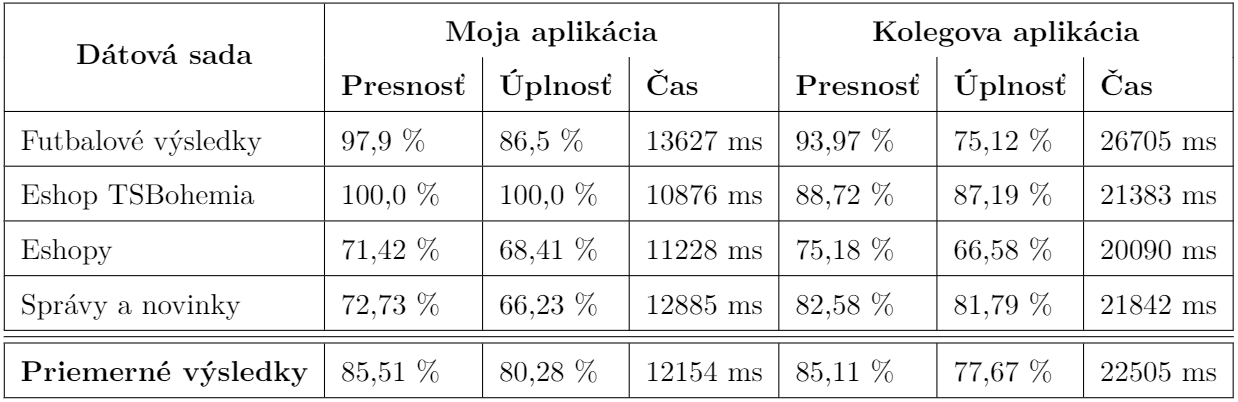
\includegraphics[width=1\textwidth]{img/vysledky.png}
    	\caption{Porovnanie dvoch odlišných prístupov k extrakcii}
    \end{figure}
\end{frame}

\bluepage{Ďakujem za pozornosť!}

\end{document}
